\documentclass{standalone}

\usepackage{ tikz }
\usetikzlibrary{bbox, automata, positioning, arrows}

\newcommand{\trs}[2]{#1 \,|\, #2}

\begin{document}
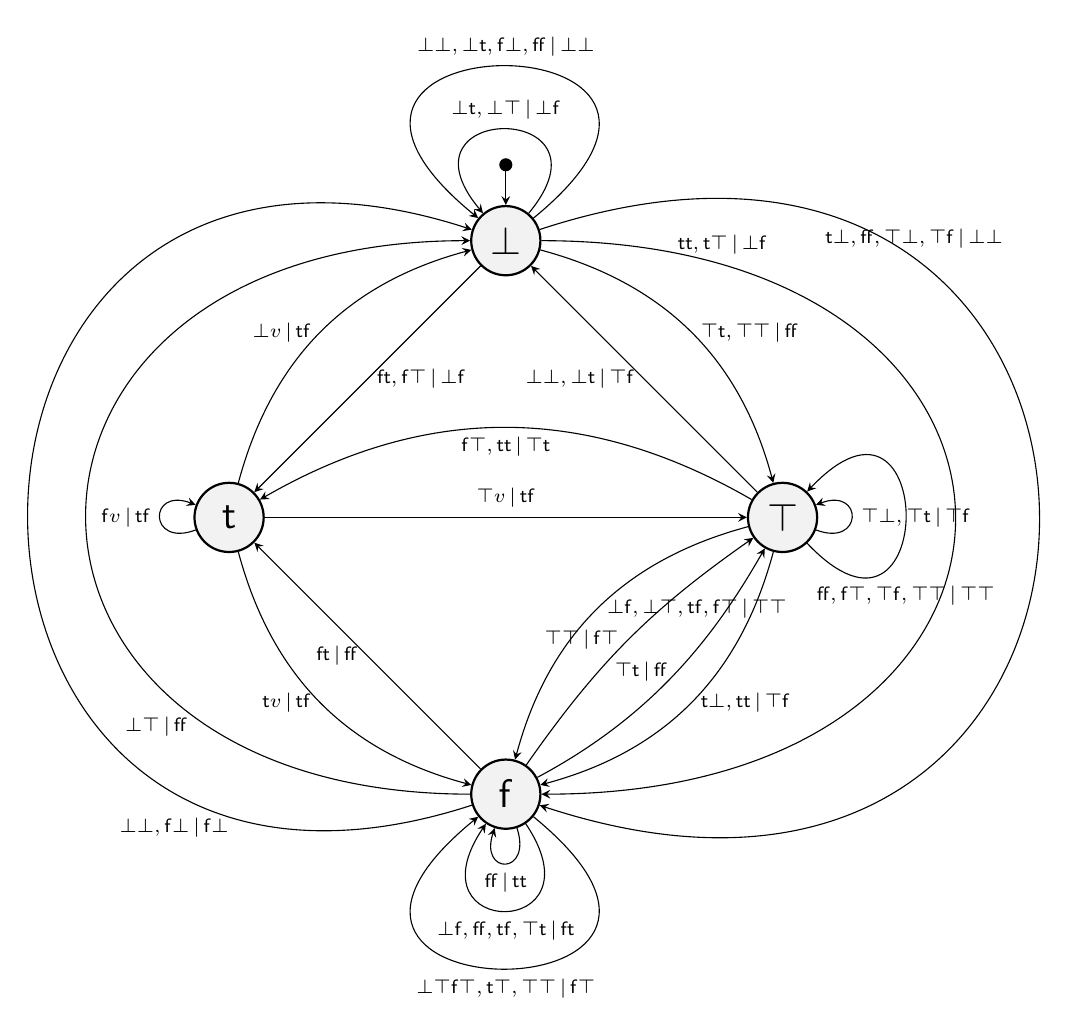
\begin{tikzpicture}[
        bezier bounding box=true,
        ->,
        >=stealth,
        node distance=0.25cm,
        every node/.style={font=\scriptsize},
        every state/.style={font=\Large, thick, fill=gray!10},
        initial text=$ $,
        initial distance=1.5cm,
        every initial by arrow/.style={*->},
        every edge/.append style={},
        yscale=-1,
        x=20pt,
        y=20pt
    ]
    \node[state, initial below] (bot) at (0,0) {\(\bot\)};
    \node[state] (true) at (-5,5) {\(\mathsf{t}\)};
    \node[state] (top) at (5,5) {\(\top\)};
    \node[state] (false) at (0,10) {\(\mathsf{f}\)};
    \draw (bot) edge[loop, out=300, in=240, distance=2.5cm] node[above]{
            \(\trs{\bot\mathsf{t},\bot\top}{\bot\mathsf{f}}\)
        } (bot);
    \draw (bot) edge[loop, out=315, in=225, distance=4.5cm] node[above] {
            \(\trs{\bot\bot,\bot\mathsf{t},\mathsf{f}\bot,\mathsf{f}\mathsf{f}}{\bot\bot}\)
        } (bot);
    \draw (bot) edge node[right]{
            \(\trs{\mathsf{f}\mathsf{t},\mathsf{f}\top}{\bot\mathsf{f}}\)
        } (true);
    \draw (bot) edge[bend right] node[right] {
            \(\trs{\top\mathsf{t},\top\top}{\mathsf{f}\mathsf{f}}\)
        } (top);
    \draw (bot) edge[distance=7cm, out=0, in=0] node[very near start, above]{
            \(\trs{\mathsf{t}\mathsf{t},\mathsf{t}\top}{\bot\mathsf{f}}\)
        } (false);
    \draw (bot) edge[distance=9cm, out=340, in=20] node[near start, above]{
            \(\trs{\mathsf{t}\bot,\mathsf{f}\mathsf{f},\top\bot,\top\mathsf{f}}{\bot\bot}\)
        } (false);
    \draw (true) edge[loop left, distance=1cm, out=135, in=225] node[left]{
            \(\trs{\mathsf{f}v}{\mathsf{t}\mathsf{f}}\)
        } (true);
    \draw (true) edge[bend right] node[left]{
            \(\trs{\bot v}{\mathsf{t}\mathsf{f}}\)
        } (bot);
    \draw (true) edge[bend left] node[left]{
            \(\trs{\mathsf{t}v}{\mathsf{t}\mathsf{f}}\)
        } (false);
    \draw (true) edge node[above]{
            \(\trs{\top v}{\mathsf{t}\mathsf{f}}\)
        } (top);


    \draw (top) edge[loop right, distance=1cm, out=45, in=315] node{
            \(\trs{\top\bot,\top\mathsf{t}}{\top\mathsf{f}}\)
        } (top);
    \draw (top) edge[loop right, distance=3cm, out=55, in=305] node[below, yshift=-0.75cm]{
            \(\trs{\mathsf{f}\mathsf{f},\mathsf{f}\top,\top\mathsf{f},\top\top}{\top\top}\)
        } (top);
    \draw (top) edge[bend left] node[below] {
            \(\trs{\mathsf{f}\top,\mathsf{t}\mathsf{t}}{\top\mathsf{t}}\)
        } (true);
    \draw (top) edge[left] node{
            \(\trs{\bot\bot,\bot\mathsf{t}}{\top\mathsf{f}}\)
        } (bot);
    \draw (top) edge[bend left] node[right]{
            \(\trs{\bot\mathsf{f},\bot\top,\mathsf{t}\mathsf{f},\mathsf{f}\top}{\top\top}\)
        } (false);
    \draw (top) edge[bend right] node[right]{
            \(\trs{\mathsf{t}\bot,\mathsf{t}\mathsf{t}}{\top\mathsf{f}}\)
        } (false);

    \draw (false) edge[loop, distance=1.5cm, out=80, in=100] node[below]{
            \(\trs{\mathsf{f}\mathsf{f}}{\mathsf{t}\mathsf{t}}\)
        } (false);
    \draw (false) edge[loop, distance=2.5cm, out=65, in=115] node[below]{
            \(\trs{\bot\mathsf{f},\mathsf{f}\mathsf{f},\mathsf{t}\mathsf{f},\top\mathsf{t}}{\mathsf{f}\mathsf{t}}\)
        } (false);
    \draw (false) edge[loop, distance=4.5cm] node[below]{
            \(\trs{\bot\top\mathsf{f}\top,\mathsf{t}\top,\top\top}{\mathsf{f}\top}\)
        } (false);
    \draw (false) edge node[left]{
            \(\trs{\mathsf{f}\mathsf{t}}{\mathsf{f}\mathsf{f}}\)
        } (true);
    \draw (false) edge[out=160, in=200, distance=8cm] node[very near start, left, xshift=-0.5cm]{
            \(\trs{\bot\bot,\mathsf{f}\bot}{\mathsf{f}\bot}\)
        } (bot);
    \draw (false) edge[distance=6.5cm, out=180, in=180] node[near start, below, xshift=-0.33cm]{
            \(\trs{\bot\top}{\mathsf{f}\mathsf{f}}\)
        } (bot);
    \draw (false) edge[out=320, in=110] node[left]{
            \(\trs{\top\mathsf{t}}{\mathsf{f}\mathsf{f}}\)
        } (top);
    \draw (false) edge[bend left, out=350, in=190] node[left]{
            \(\trs{\top\top}{\mathsf{f}\top}\)
        } (top);
\end{tikzpicture}
\end{document}